\section{Анализ отдельных примеров}

\subsection{Роль анализа отдельных примеров в работе}

После построения предиктивного ядра, перехода к рекомендательной постановке, анализа уверенности и слоя интерпретации
возникает задача показать, как система ведёт себя не только на уровне усреднённых метрик, но и на уровне отдельных
наблюдений. Для этого в работе используются специально отобранные примеры полей, на которых можно последовательно
проследить связь между историей культур, результатом модели, уровнем уверенности и графовым интерпретационным
контекстом.

Такой формат анализа важен по двум причинам. Во-первых, усреднённые метрики не показывают, как именно ранжированный
список кандидатов работает в простых и сложных случаях. Во-вторых, слой интерпретации по своей природе является
локальным: его смысл раскрывается не на уровне общей таблицы результатов, а на уровне конкретного списка кандидатов для
конкретного поля. Поэтому анализ отдельных примеров в данной работе выступает как естественный способ показать, каким
образом предиктивный слой, слой оценки уверенности и графовый слой взаимодействуют между собой.

В проекте были собраны четыре примера:

\begin{itemize}
\tightlist
\item
  с высокой уверенностью;
\item
  со средней уверенностью;
\item
  с низкой уверенностью;
\item
  сложный пример с расхождением сигналов.
\end{itemize}

Этот набор позволяет охватить как относительно простые и устойчивые сценарии, так и случаи, где ранжированный список
кандидатов требует более внимательной интерпретации.

Сводка выбранных примеров приведена в таблице~\ref{tab:case-studies-summary}. Каждый пример соответствует одному
конкретному наблюдению из тестового фрагмента, для которого известны фактическая следующая культура, список из трёх
кандидатов модели и оценки слоя интерпретации на уровне отдельных кандидатов. Поэтому далее сравниваются не абстрактные
типы ситуаций, а конкретные культуры-кандидаты: например, \texttt{forage\_hay}, \texttt{corn}, \texttt{legumes},
\texttt{soybeans} и их альтернативы внутри ранжированного списка.

\begin{table}[H]
\centering
\scriptsize
\caption{Содержательная сводка case studies}
\label{tab:case-studies-summary}
\setlength{\tabcolsep}{1.5pt}
\begin{tabular}{@{}>{\raggedright\arraybackslash}p{0.14\textwidth}
                >{\raggedright\arraybackslash}p{0.11\textwidth}
                >{\raggedright\arraybackslash}p{0.20\textwidth}
                >{\raggedright\arraybackslash}p{0.15\textwidth}
                >{\raggedright\arraybackslash}p{0.15\textwidth}
                >{\raggedright\arraybackslash}p{0.19\textwidth}@{}}
\toprule
Case & Фактическая культура & Top-3 CatBoost & Самый поддержанный KG кандидат & Статус & Ключевой вывод \\
\midrule
High confidence
  & \texttt{forage\_hay}
  & \texttt{forage\_hay} ($p_1=0.930$), \texttt{corn}, \texttt{wheat}
  & \texttt{forage\_hay} ($gs=0.661$)
  & top-1 верен; target в Top-3; alignment strong
  & модель и KG согласованы: фактическая культура совпадает с top-1 и имеет сильную графовую поддержку \\
Medium confidence
  & \texttt{corn}
  & \texttt{corn} ($p_1=0.669$), \texttt{soybeans}, \texttt{forage\_hay}
  & \texttt{soybeans} ($gs=0.508$)
  & top-1 верен; target в Top-3; alignment weak
  & модель выбирает правильный \texttt{corn}, но KG сильнее поддерживает \texttt{soybeans}; это пример конкурирующей
  альтернативы внутри shortlist \\
Low confidence
  & \texttt{legumes}
  & \texttt{legumes} ($p_1=0.432$), \texttt{soybeans}, \texttt{fallow}
  & \texttt{soybeans} ($gs=0.568$)
  & top-1 верен; target в Top-3; alignment weak
  & top-1 совпал с target, но модельная уверенность и graph support для него низкие; результат лучше читать как
  shortlist, а не как жёсткое предписание \\
Difficult class
  & \texttt{soybeans}
  & \texttt{corn} ($p_1=0.689$), \texttt{cotton}, \texttt{soybeans}
  & \texttt{soybeans} ($gs=0.386$)
  & top-1 неверен; target в Top-3; alignment weak
  & фактическая культура не первая, но остаётся в shortlist; KG выделяет её как более семантически поддержанную
  альтернативу \\
\bottomrule
\end{tabular}

\vspace{0.4em}
\footnotesize $p_1$ --- вероятность top-1 кандидата CatBoost; $gs$ --- \texttt{graph\_support\_score}.
Источники: \path{artifacts/results/knowledge_graph_explainability/case_summary.csv},
\path{artifacts/results/knowledge_graph_explainability/case_explanations.csv}.
\normalsize
\end{table}


\subsection{Пример с высокой уверенностью}

Первый тип примеров соответствует ситуациям, в которых модель демонстрирует высокий уровень уверенности, а первая
рекомендация выглядит содержательно согласованной с интерпретационным контекстом. В таких случаях история поля,
вероятностный вывод модели и графовая поддержка обычно не противоречат друг другу. Это наиболее простой сценарий работы
системы: ранжированный список остаётся полезным, но первая позиция уже выглядит достаточно устойчивой.

В рассматриваемом примере с высокой уверенностью фактической следующей культурой является \texttt{forage\_hay}, и
CatBoost также ставит \texttt{forage\_hay} на первое место с вероятностью 0.930. Граф знаний не предлагает более
сильную альтернативу: наиболее поддержанным кандидатом также остаётся \texttt{forage\_hay}. Поэтому этот пример
показывает согласованный сценарий, где модельная оценка, фактический целевой класс и графовая поддержка сходятся в одной
культуре.

С точки зрения интерпретации этот пример показывает поведение системы в условиях
относительно устойчивого паттерна. Если поле относится к хорошо распознаваемой структуре, модель формирует сильную
первую рекомендацию, а графовый слой показывает, что выбранный кандидат поддержан переходной статистикой,
региональным контекстом и активными правилами.

\subsection{Пример со средней уверенностью}

Второй тип примеров соответствует случаям средней уверенности. Здесь первая рекомендация остаётся содержательно
правдоподобной, однако ранжированный список в целом становится более важным, поскольку помимо первой позиции появляются и
другие кандидаты, которые могут выглядеть осмысленно с точки зрения истории поля и интерпретационного контекста.

В примере со средней уверенностью фактической культурой является \texttt{corn}, и модель правильно помещает
\texttt{corn} на первую позицию. Однако графовый сигнал сильнее поддерживает альтернативу \texttt{soybeans}: для неё
выше \texttt{graph\_support\_score}, а в объяснении присутствует поддержка через \texttt{legume\_break\_bonus} и
региональную типичность. Поэтому этот пример показывает ситуацию, где первая рекомендация формально верна, но
ранжированный список содержит содержательно конкурирующую альтернативу.

Этот пример раскрывает прикладной смысл рекомендательной постановки: она полезна не только для обработки явных и простых
ситуаций, но и для анализа наблюдений, где система не должна ограничиваться одним ответом. В подобных случаях ранжированный список играет роль пространства разумных альтернатив: модель указывает
основное направление, а граф знаний позволяет рассматривать соседние варианты как содержательно поддержанные кандидаты.

\subsection{Пример с низкой уверенностью}

Третий тип примеров связан со случаями низкой уверенности. Именно такие наблюдения особенно хорошо показывают, почему
слой оценки уверенности и рекомендательная постановка с несколькими кандидатами являются принципиально важными для всей
системы. В подобных сценариях первая рекомендация может быть недостаточно устойчивой, однако ранжированный список в
целом остаётся полезным, поскольку в нём по-прежнему присутствуют правдоподобные альтернативы.

В примере с низкой уверенностью фактическая культура --- \texttt{legumes}. Модель ставит \texttt{legumes} на первое
место, но с заметно меньшей вероятностью 0.432. При этом граф знаний сильнее поддерживает \texttt{soybeans}, то есть
близкую по смыслу альтернативу из группы бобовых. Такой пример важен именно потому, что первая рекомендация оказалась
правильной, но её нельзя интерпретировать как устойчивое однозначное решение: и уровень уверенности, и графовая
поддержка указывают на спорность ситуации.

На уровне интерпретации это проявляется в том, что графовый контекст может поддерживать не только первую рекомендацию,
но и одну или несколько альтернатив. Для пользователя это означает, что результат не следует воспринимать как сильное
однозначное предписание. Напротив, низкая уверенность должна побуждать рассматривать несколько кандидатов одновременно и
использовать дополнительный предметный анализ.

\subsection{Сложный пример с расхождением сигналов}

Четвёртый тип примеров соответствует наиболее сложным ситуациям, в которых наблюдается напряжение между первой
рекомендацией модели и интерпретационным контекстом. Именно такие случаи позволяют лучше всего показать, зачем в
архитектуре нужен графовый слой. В этих сценариях первая позиция списка кандидатов может не совпадать с наиболее сильно
поддержанным графом кандидатом, а фактическая следующая культура может находиться не на первом месте, а среди
альтернатив в списке из трёх кандидатов.

В сложном примере фактической культурой является \texttt{soybeans}, тогда как первая рекомендация модели ---
\texttt{corn} с вероятностью 0.689. При этом \texttt{soybeans} всё же присутствует в списке из трёх кандидатов на
третьей позиции и получает более сильную поддержку со стороны графа знаний, чем первая рекомендация.
Именно этот пример наиболее явно показывает ценность рекомендательной постановки: первая рекомендация оказывается ошибочной,
но ранжированный список и слой интерпретации сохраняют полезную информацию о фактическом целевом классе.

На рисунке~\ref{fig:difficult-case-subgraph} показан локальный подграф интерпретации для данного примера. Он отражает
связи между кандидатами, региональным контекстом, группами культур и правилами, которые формируют графовую поддержку.

\begin{figure}[H]
    \centering
    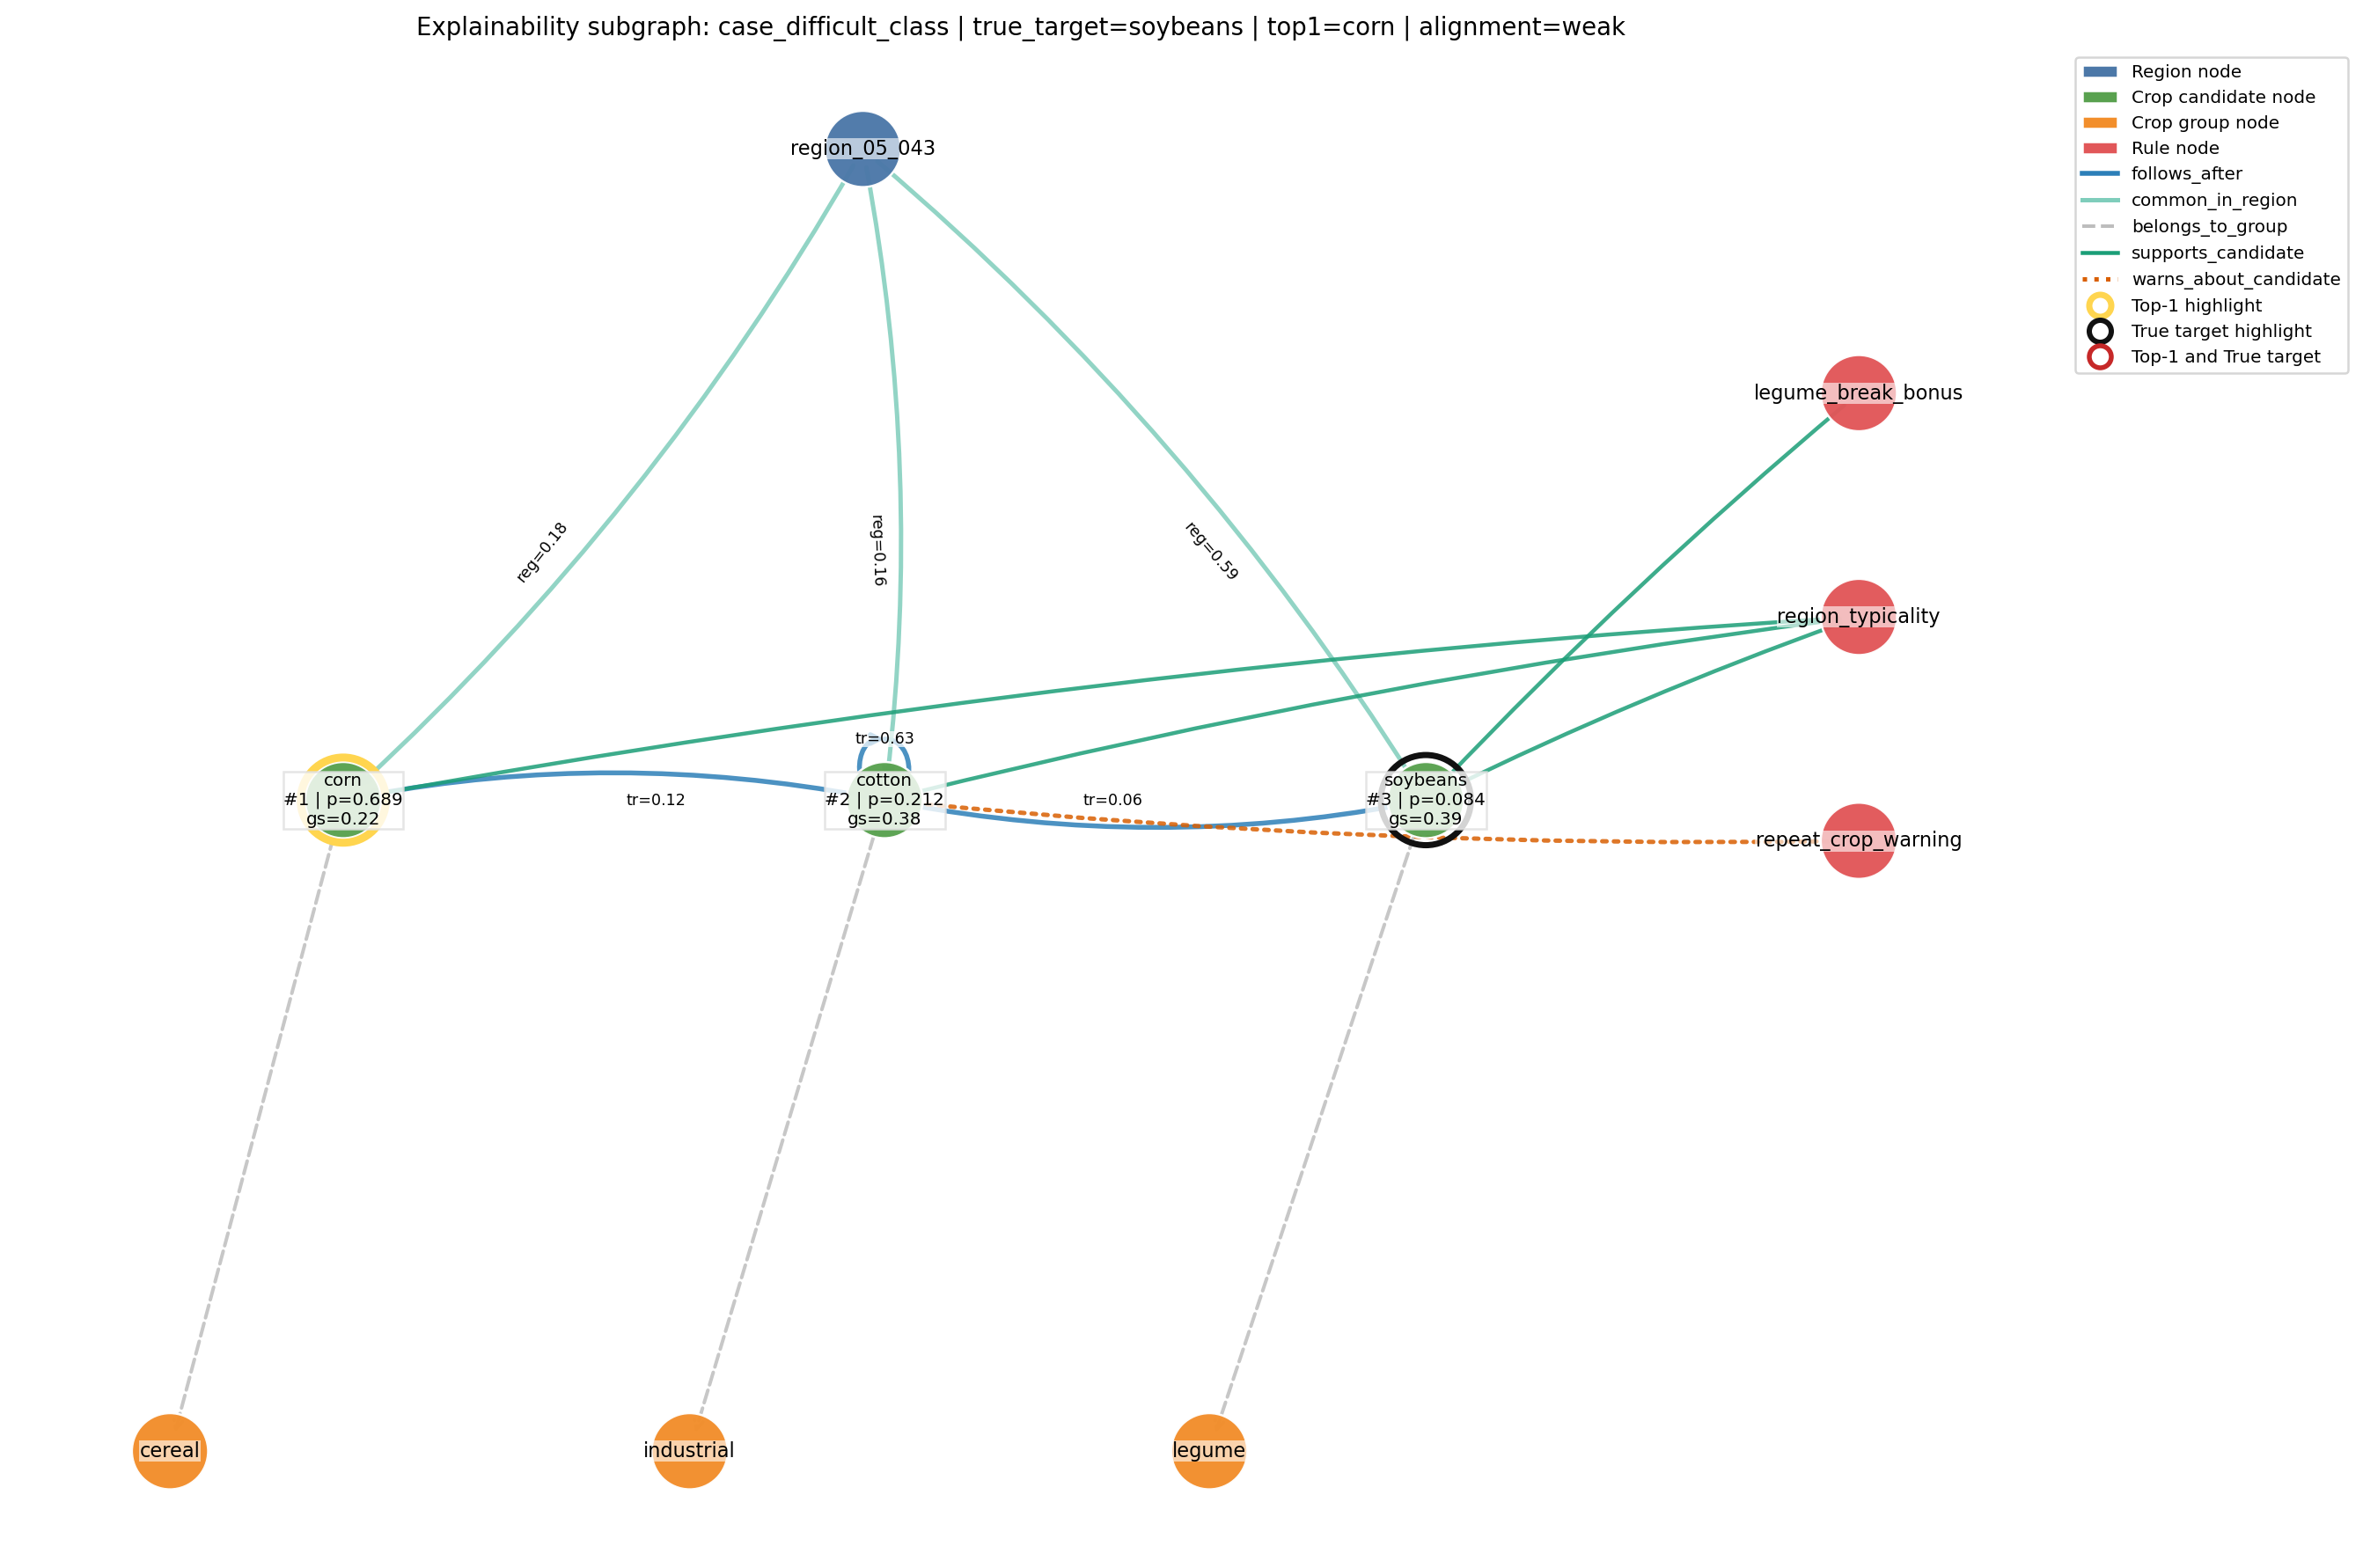
\includegraphics[width=0.95\textwidth]{figures/case_difficult_class.png}
    \caption{Подграф интерпретации для сложного примера с расхождением модельного и графового сигналов}
    \label{fig:difficult-case-subgraph}
\end{figure}

Из рисунка видно, что первая рекомендация модели и фактическая культура относятся к разным частям интерпретационного
контекста. При этом \texttt{soybeans}, несмотря на третью позицию в модельном ранжировании, получает более высокую
графовую поддержку, чем \texttt{corn}. Это иллюстрирует, почему в сложных случаях важно анализировать не только первую
рекомендацию, но и весь короткий список кандидатов.

Краткая сводка сложного примера в формате карточки приведена в таблице~\ref{tab:difficult-case-card}.

\begin{table}[H]
\centering
\small
\caption{Difficult-case: краткая карточка наблюдения}
\label{tab:difficult-case-card}
\setlength{\tabcolsep}{4pt}
\renewcommand{\arraystretch}{1.12}
\begin{tabular}{|>{\raggedright\arraybackslash}p{0.36\textwidth}|>{\raggedright\arraybackslash}p{0.58\textwidth}|}
\hline
Параметр & Значение \\
\hline
История поля & \texttt{corn $\rightarrow$ corn $\rightarrow$ cotton} \\
\hline
\texttt{true\_target} & \texttt{soybeans} \\
\hline
Top-1 модели / вероятность / уверенность & \texttt{corn}, $p_1 = 0.6887$, \texttt{medium\_confidence} \\
\hline
\texttt{true\_target} в shortlist & Да \\
\hline
Shortlist (Top-3) & \texttt{corn} (0.6887), \texttt{cotton} (0.2118), \texttt{soybeans} (0.0835) \\
\hline
Лучший кандидат по graph support & \texttt{soybeans} \\
\hline
Graph support (best candidate) & 0.3863 \\
\hline
Интерпретация
    & Сложный кейс: top-1 ошибается, но \texttt{true\_target} присутствует в shortlist и сильнее поддержан графом. \\
\hline
\end{tabular}

\vspace{0.4em}
\footnotesize Источники: \path{artifacts/results/knowledge_graph_explainability/case_summary.csv},
\path{artifacts/results/knowledge_graph_explainability/case_explanations.csv},
\path{notebooks/09_knowledge_graph_explainability.ipynb}.
\normalsize
\end{table}

Интерпретация таких случаев особенно важна. Их не следует трактовать как прямое противопоставление модели и графа знаний.
Их смысл заключается в другом: ранжированный список следует рассматривать как пространство конкурирующих вариантов, где
первая позиция не всегда исчерпывает всю полезную информацию. Если слой интерпретации сильнее поддерживает
альтернативного кандидата, это указывает на спорность ситуации и делает анализ примера более содержательным.

\subsection{Общая интерпретация рассмотренных примеров}

Рассмотренные примеры позволяют сделать несколько важных выводов. Во-первых, они подтверждают рекомендательную природу
прототипа, полезность которого особенно проявляется в анализе нескольких кандидатов одновременно. Во-вторых, они
показывают, что слой оценки уверенности
действительно задаёт различие между более устойчивыми и более спорными рекомендациями. В-третьих, они демонстрируют,
что граф знаний дополняет модельный результат и помогает интерпретировать различия между кандидатами внутри ранжированного списка.

Таким образом, анализ отдельных примеров в работе выполняет не иллюстративную, а аналитическую функцию. Он связывает
между собой историю поля, ранжированный список кандидатов, сигнал уверенности и графовый интерпретационный контекст.

Рассмотренные примеры показывают работу базовой версии графа знаний. Далее на тех же случаях анализируется, как меняется
интерпретационный контекст после добавления литературных правил.
